\title{Midterm 2 for Electromagnetic Theory (PHYS330)}
\author{Dr. Jordan Hanson - Whittier College Dept. of Physics and Astronomy}
\date{\today}
\documentclass[10pt]{article}
\usepackage[a4paper, total={18cm, 27cm}]{geometry}
\usepackage{amsmath}
\usepackage{graphicx}
\usepackage{hyperref}
\begin{document}
\twocolumn
\maketitle

\begin{figure}
\centering
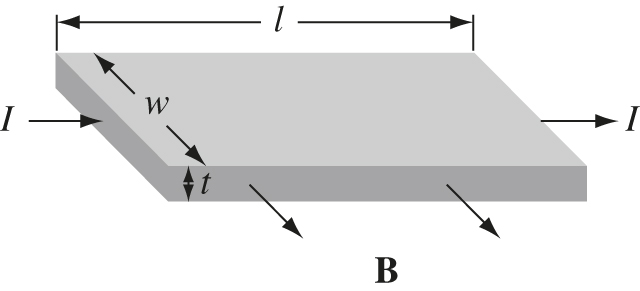
\includegraphics[width=0.3\textwidth]{figures/5_59.jpg}
\caption{\label{fig:1} A rectangular bar of metal of length $l$, width $w$, current $I$, in a perpendicular field $\mathbf{B}$.}
\end{figure}

\begin{figure}
\centering
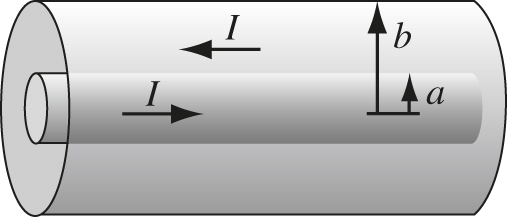
\includegraphics[width=0.2\textwidth]{figures/6_24.jpg}
\caption{\label{fig:2} A coaxial cable system with magnetic susceptibility $\chi_{\rm m}$ between the inner and outer conductors.}
\end{figure}

\begin{abstract}
This exam may be completed at home, and covers chapters 5-7 of the course text and in-class examples.  Class notes and the course text may be used for review.  The course warm-up exercises are good study materials for this exam.
\end{abstract}
\noindent

\section{Chapter 5}

\begin{enumerate}
\item Using the Biot-Savart Law, show that the $\mathbf{B}$-field at the center of a circular loop of wire in the xy-plane, centered at the origin, is $\mathbf{B} = \mu_0 I/(2 R)\hat{\mathbf{z}}$.
\item The magnetic dipole moment of a loop of current is define like:
\begin{equation}
\mathbf{m} = I\int d\mathbf{a}
\end{equation}
(a) Suppose a circular loop of current with radius $b$ lies in the xy-plane, centered at the origin.  Calculate $\mathbf{m}$. (b) Suppose the loop is \textit{tilted}, such that $\mathbf{m}$ makes a small angle $\theta_0$ with respect to the z-axis.  Calculate the torque in terms of given parameters. (c) If released from $\theta_0$, derive the equation of motion describing the direction of $\mathbf{m}$.
\item A current $I$ flows to the right through a rectangular bar of metal, with a uniform $\mathbf{B}$-field (Fig. \ref{fig:1}). (a) If the moving charges are positive, in which direction are the deflected by $\mathbf{B}$? (b) The deflection results in an accumulation of charge on the upper and lower surfaces of the bar, which in turn produces an electric force to counteract the magnetic one.  Equilibrium occurs when the forces cancel.  Find the voltage between the top and bottom of the bar, in terms of $B$, $v$ (speed of charges), and bar dimensions. (c) What would the voltage be if the moving charges were negative?
\end{enumerate}

\section{Chapter 6}

\begin{enumerate}
\item A coaxial cable consists of two very long cylindrical tubes, separated by linear insulating material of magnetic susceptibility $\chi_{\rm m}$.  A current $I$ flows down the inner conductor and returns along the outer one; in each case, the current distributes itself uniformly over the surface (Fig. \ref{fig:2}).  (a) Find the magnetic field in the region between the tubes.  (b) As a check, calculate the $\mathbf{M}$ and the bound currents, and confirm that (together with the free currents) they generate the correct field.
\item (a) Use Amp\`{e}re's Law to generate the formula for the $\mathbf{B}$-field of a long cylindrical solenoid. (b) Now add an iron bar inside the solenoid that fills the volume.  Derive the new expression for the $\mathbf{B}$-field in terms of magnetic susceptibility.  (c) Look up the relative permeability of iron, and calculate the value of $\mathbf{B}$ for $I = 1$ amp, and $n=10$ turns per cm.
\end{enumerate}

\section{Chapter 7}

\begin{enumerate}
\item A metal bar of mass $m$ slides frictionlessly on two parallel conducting rails a distance $l$ apart (Fig. \ref{fig:3}, left)).  A resistor $R$ is connected across the rails, and a uniform magnetic field $\mathbf{B}$ (into the page) fills the region. (a) If the bar moves to the right with speed $v$, what is the current in the resistor? (b) What is the magnetic force vector on the bar? (c) If the bar begins with initial speed $v_i$, it has kinetic energy $(1/2) m v_i^2$.  Check that the energy delivered to the resistor is equal to the initial kinetic energy.
\item A square loop is mounted on a vertical shaft and rotated at angular velocity $\omega$.  A uniform magnetic field $\mathbf{B}$ points to the right.  Find the AC voltage for the terminals at the bottom.
\end{enumerate}

\begin{figure}[hb]
\centering
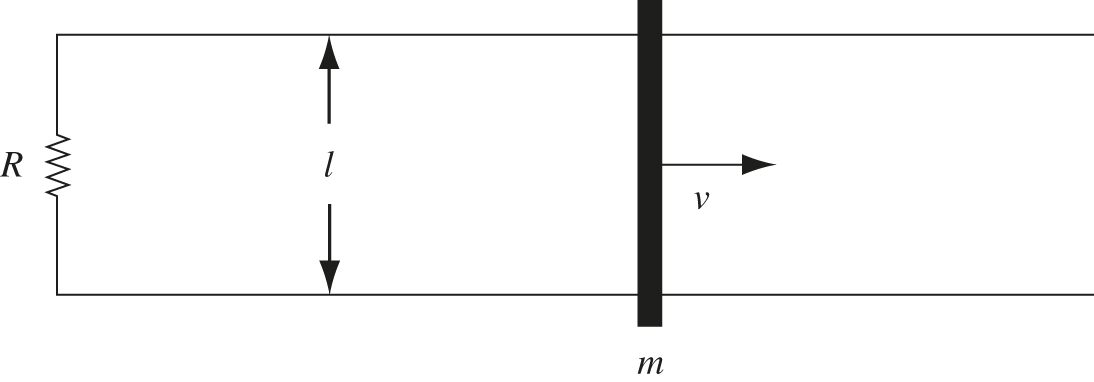
\includegraphics[width=0.33\textwidth]{figures/7_17.jpg} \hspace{0.2cm}
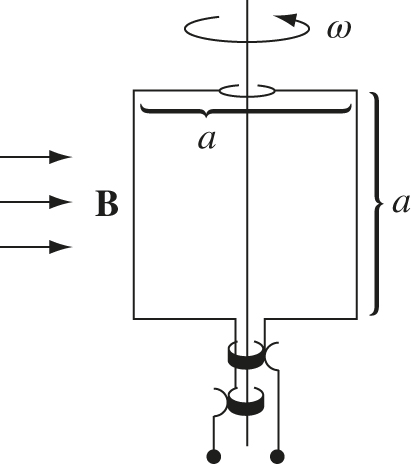
\includegraphics[width=0.125\textwidth]{figures/7_19.jpg}
\caption{\label{fig:3} (Left) A bar can slide on rails in a $\mathbf{B}$ field. (Right) A model of an AC generator.}
\end{figure}

\end{document}
